\chapter{Perancangan}
\label{chap:perancangan}

\section{Diagram Kelas Rinci} 
\label{sec:diagram_kelas_rinci}
Diagram kelas rinci diperoleh dari hasil pengembangan diagram kelas analisis pada subbab \ref{sec:analisis_kelas}. Diagram kelas rinci dapat dilihat pada gambar \ref{fig:final_class_diagram}. Rincian kelas beserta fungsinya

\section{Perancangan Antarmuka}
\label{sec:perancangan_antarmuka}

Untuk memenuhi kebutuhan interaksi antara pengguna dengan sistem, maka dirancanglah sebuah antarmuka dari Informatika Student Portal. Rancangan antarmuka dibagi menjadi lima halaman web antara lain:

\begin{enumerate}
	\item {Antarmuka Halaman \textit{Login}}\\
	Halaman ini digunakan untuk melakukan \textit{login}. Komponen halaman ini terdiri dari logo aplikasi, kolom \textit{email}, kolom \textit{password}, dan tombol \textit{login} seperti yang ditunjukkan pada gambar \ref{fig:4_ranc_login}. Untuk melakukan \textit{login}, pengguna perlu memasukkan \textit{email} dan \textit{password} yang sesuai kemudian menekan tombol \textit{login}. Jika berhasil pengguna akan diarahkan ke halaman \textit{home}. 
		\begin{figure}[H]
			\centering
			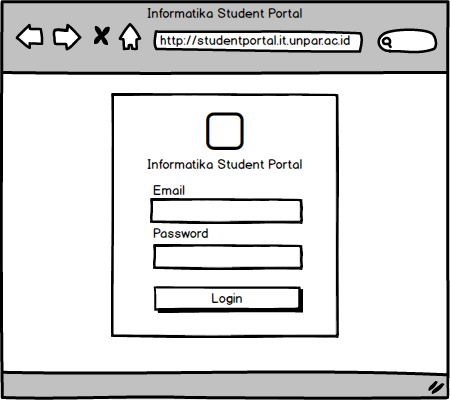
\includegraphics[scale=0.5]{Gambar/Login_Page}
			\caption{Rancangan Halaman \textit{Login}} 
			\label{fig:4_ranc_login}
		\end{figure}
		
	\item {Antarmuka Halaman \textit{Home}}\\
	Halaman \textbf{home} merupakan halaman yang pertama dituju setelah melakukan \textbf{login}. Halaman ini, menampilkan identitas pengguna seperti foto profil, nama, Nomor Induk Mahasiswa(NPM), dan \textit{email} mahasiswa. Rancangan antarmuka halaman \textit{home} dapat dilihat pada gambar \ref{fig:4_ranc_home}.
		\begin{figure}[H]
			\centering
			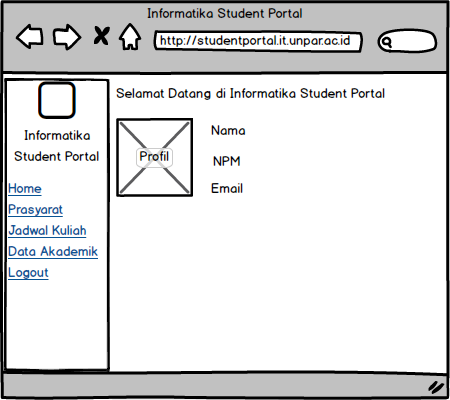
\includegraphics[scale=0.5]{Gambar/Home_Page}
			\caption{Rancangan Halaman \textit{Home}} 
			\label{fig:4_ranc_home}
		\end{figure}
		
	\item {Antarmuka Halaman Prasyarat Mata Kuliah}\\
	Halaman ini menampilkan tabel prasyarat mata kuliah yang dibuka pada semester terkini. Tabel tersebut memiliki tiga kolom yaitu kode mata kuliah, nama mata kuliah, dan status pengambilan mata kuliah. Rancangan antarmuka halaman prasyarat mata kuliah dapat dilihat pada gambar \ref{fig:4_ranc_prasyarat}.
	\begin{figure}[H]
			\centering
			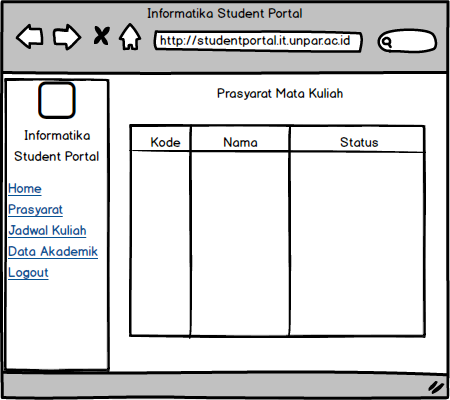
\includegraphics[scale=0.5]{Gambar/Prasyarat_Page}
			\caption{Rancangan Halaman Prasyarat Mata Kuliah} 
			\label{fig:4_ranc_prasyarat}
		\end{figure}
	\item {Antarmuka Halaman Jadwal Kuliah}\\
	Halaman ini menampilkan jadwal kuliah semester terkini yang tersusun dan terurut berdasarkan hari. Rancangan antarmuka halaman jadwal kuliah dapat dilihat pada gambar \ref{fig:4_ranc_kuliah}.
	\begin{figure}[H]
			\centering
			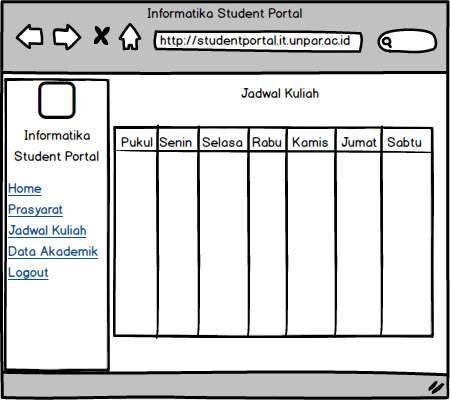
\includegraphics[scale=0.5]{Gambar/Jadwal_Page}
			\caption{Rancangan Halaman Jadwal Kuliah} 
			\label{fig:4_ranc_kuliah}
		\end{figure}
	\item {Antarmuka Halaman Data Akademik}\\
	Halaman ini menampilkan ringkasan informasi akademik pengguna yaitu IPS semester terakhir, IPK, SKS lulus, sisa SKS menuju kelulusan, dan status pengambilan mata kuliah pilihan wajib. Rancangan antarmuka halaman data akademik dapat dilihat pada gambar \ref{fig:4_ranc_ringkasan}.
	\begin{figure}[H]
			\centering
			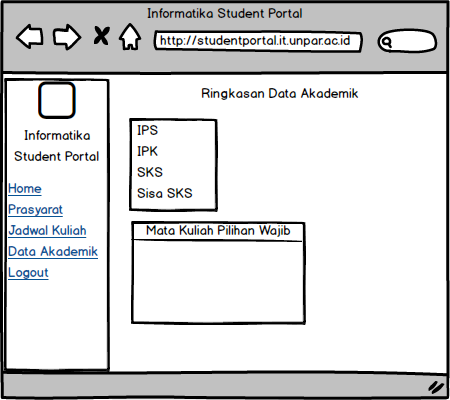
\includegraphics[scale=0.5]{Gambar/Ringkasan_Page}
			\caption{Rancangan Halaman Data Akademik} 
			\label{fig:4_ranc_ringkasan}
		\end{figure}
\end{enumerate}
